
\clearpage
\renewcommand{\theequation}{S.\arabic{equation}}
\renewcommand{\thesection}{S.\arabic{section}}
\setcounter{section}{0}
\setcounter{equation}{0}
% \setcounter{page}{1}
% \pagenumbering{roman}

%----------------------------------------------------------------------------------------
%	Supp
%----------------------------------------------------------------------------------------
\section*{Supplemental Material}

One challenge to establishing proportionality in mixed-member (MM) systems is that there is no fair or practical way of \emph{removing} representatives from parties that are over-represented.
Seats can be added, however, and so the additional member system (AMS) is another common name that highlights how MPs are added to an existing body to approach proportionality.
Generally, the D'Hondt highest averages method is used for this process, which we briefly review now. None of the mathematical details presented here are necessary for the average voter to either (a) cast their ballot, or (b) appreciate the correspondence in proportionality between popular vote and final seat distribution.

Assume a parliamentary body must represent $N$ constituencies, after an election involving $M$ major parties. A `major' party is defined as any party whose popular support exceeds the 5\% threshold on the 2nd ballot\footnote{Minor parties are ignored, so unless otherwise stated, `major' is implied. Likewise, a vote for a `party' refers to the 2nd ballot.}.
The index  $m \in \left\{0, .., M-1\right\} $  denotes party, and for each party $m$, a list of quotients $Q_{m,j}$ are defined as

\begin{equation}
\label{eq:DhondtSupp}
Q_{m,j} = \frac{V_m}{j},
\end{equation}

where $j \in \left\{ 1,.., \infty \right\}$ is an index\footnote{Conventionally, this might be written as $j+1$ in the denominator, with initial value $j=0$; the above has been chosen with initial value $j=1$ for readability}, and  $V_m$ is the number of votes for party $m$, out of a total of $\hat{V}$. Let $V^I$ denote the sum of 2nd ballots that were either spoiled, or cast for minor parties that failed to meet the 5\% threshold, thus:
\begin{equation}
\label{eq:sum_Vm}
V^I + \sum_m V_m = \hat{V}.
\end{equation}
Let $C_m$ represent the number of direct constituent seats that party $m$ was awarded from the total $N$, and $C^I$ the number of seats won by independent candidates, or candidates from minor parties,
\begin{equation}
\label{eq:sum_Cm}
C^I + \sum_m C_m = N.
\end{equation}

In practice, $C_m$ and $V_m$ will clearly be correlated, since voters tend to prefer candidates and parties along similar ideological lines. However, since $C_m$ is determined entirely by the first ballot, and $V_m$ refers exclusively to the second, these quantities are, in principle, independent.

The D'Hondt highest averages method is predicated on the assumption that for a parliament of size $\hat{N}$, the largest $\hat{N}$ quotients are awarded seats.
For reasons described in the main text, we seek the smallest value of $\hat{N}$ for which this is possible, while still including all candidates directly elected from a constituency.
Clearly this will require $\hat{N}\ge N$, and each party will be awarded a number of supplementary seats $S_m$ (as yet undetermined) to establish their total seat count

\begin{equation}
\label{eq:sum_Sm}
C^I + \sum_m\left( S_m +C_m\right) = \hat{N} \ge N.
\end{equation}

%-----------
The index $m$ is arbitrary, and thus we define it in order of relative constituent representation. That is to say, $m=0$ refers to the most initially over-represented party:
\begin{align}
\label{eq:most_overrep}
\frac{C_0/N}{V_0/\hat{V}} &\ge& \frac{C_m/N}{V_m/\hat{V}}, \\
\frac{C_0}{V_0} &\ge& \frac{C_m}{V_m} && \forall \,\, m.
\end{align}

The quotient $Q_{0,C_0}$ is then the lowest quotient that corresponds to a constituent seat. To see this, note that from \ref{eq:DhondtSupp}, we have

\begin{equation}
\label{eq:QmCm}
Q_{m,C_m} = \frac{V_m}{C_m} \ge \frac{V_0}{C_0} \,  \forall \, m,
\end{equation}
where all $C_m,V_m$ are positive integers. For proportionality, we must then allocate an additional $S_m$ seats to each party $m \neq 0$. If quotients are selected until the  threshold defined by $Q_{0,C_0}$ is met, we are left with

\begin{align}
\label{eq:QmSm}
Q_{m,C_m+S_m} = \frac{V_m}{C_m+S_m} &\to& \frac{V_0}{C_0}^+ \\
{C_m+S_m} &\to& \frac{V_mC_0}{V_0}^-.
\end{align}

To see how this imposes proportionality, first consider the simplified case where $C^I=V^I=0$ (i.e., no seats won by independent candidates, and all 2nd ballot votes cast for major parties). Here, party $m$'s share of seats approaches:

\begin{align}
\label{eq:seatshare}
\frac{C_m+S_m}{ \sum\limits_k\left( C_k+S_k \right)} &\to& \frac{V_m C_0/V_0^-}{ \sum\limits_k V_k C_0/V_0^-} \\
&\to& \frac{V_m}{\hat{V}}^-,
\end{align}
that is, party $m$'s share of the popular vote (rounded down to the nearest integer)..

This simplified case is actually not far removed from recent elections, where independent seats are relatively rare ($C^I\approx0$), and minor parties have obtained only a few percentage points of popular support ($V^I \approx 0$).
%Nevertheless, our proposal must be robust and precise. %-- omitted.
Accounting for independent seats and votes, however, requires subtle discussion that is not limited to mathematics, as we will see in the following section.

%----------------------------------------------------------------------------------------
%	Independent and spoiled
%----------------------------------------------------------------------------------------

\section{Independent and Spoiled Ballots}
\label{sec:outliers}
Consider a hypothetical minimal election with 100 total ballots, 95 of which were valid, the other five of which were spoiled. Suppose party $X$ obtained 45 votes and remained under-represented against parties $Y$ and $Z$, who together obtained another 45 votes. The remaining 5 valid votes were cast for various small parties ($\alpha,\beta,$ etc. \ldots), each of which fell below the 5\% threshold required for supplementary seats.
What then is the `proportional' share of seats for party $X$?
Traditional MM would suggest 50\% ($X$'s share of the valid major-party votes, 45/90), as supplemental seats are shared only among major parties. Alternatively, one might interpret `proportionality' to mean 47\% ($X$'s share of valid votes, 45/95), or 45\% ($X$'s share of the voting electorate, 45/100).


In the 2011 election, for example, both the NDP and Liberal parties were under-represented; it is difficult to argue that someone who voted for the Rhinoceros party, for example, would want their share of the popular vote used to provide compensatory seats to either the NDP or Liberal parties \--indeed, such a voter explicitly voted \emph{against} these parties.
Nor did this voter support the over-represented Conservative party, either, however each of the Conservative Party’s seats has another justification based on constituency representation.
As far as supplementary seating is concerned (the purpose of which is establishing proportionality), this voter’s share of the popular vote cannot fairly be used by \emph{any} major party.

This is especially true if such a minor party won constituency seats. For example, in both 2011 and 2015 the Green Party failed to obtain 5\% of the popular vote and therefore would not qualify for supplementary seats. The Green Party did, however, obtain a single constituency seat, and therefore, \emph{any} additional MPs would serve to diminish the relative power of the Green Party's lone representative.
As such, the Green Party’s share of popular votes (3.9\% in 2011, 3.5\% in 2015) can hardly be used towards proportionality for other competing underrepresented parties. What then should be done with the corresponding 3.9\% (or 3.5\%) of seats in parliament? 
A parsimonious approach would suggest that the share of valid 2nd ballot votes cast for minor parties should be agnostic with respect to major parties, and default towards the existing FPP result from the 1st ballot. Such ballots then serve to inhibit \emph{all} major parties from obtaining supplementary seats.

Spoiled ballots present a different issue, but similar logic applies: some voters may wish to vote \emph{only} for their local candidate, without supporting \emph{any} existing party (e.g. if they are voting for an independent candidate).
A voter who supports only that candidate would wish to prevent the addition of any supplementary MPs to avoid diluting their representative's power once in office; a spoiled 2nd ballot might then represent a legitimate wish to obstruct the addition of \emph{any} supplemental MPs.

Given these considerations, for the above hypothetical election, PMM takes the approach that if party $X$ receives 45\% of the total ballots \--\emph{including spoiled ballots and ballots cast for minor parties}\-- then it is entitled to 45\% of the parliamentary seats.
Spoiled, and minor-party 2nd ballots should default towards the preexisting results from the first ballot (i.e., the current FPP system), and serve to inhibit supplementary MPs altogether.
In practice, recent elections suggest that these votes usually comprise about 2-4\% of ballots. Counting \emph{everyone} means counting them as well.

With these considerations in mind, the algorithm remains very much the same as in the standard D'Hondt process, however the termination criterion is slightly different.

\begin{enumerate}
\item All FPP winners from 1st ballots are assigned seats.
Each major party seat is associated with a quotient from their party's list, in order. The remaining quotients from all parties are then sorted in a new list.

\item Proceeding through this list in order (starting with $S_m=0 \, \forall \, m$), we may calculate the number of seats that is owed to the party associated with the quotient in question:
\begin{align}
\left(\frac{V_m}{\hat{V}}\right) \hat{N} -(C_m+S_m)\stackrel{?}{\ge} 1.
\label{eq:Qowed1seat}
\end{align}

One might read the left side of Eq.~\ref{eq:Qowed1seat} as `the number of seats party $m$ should expect, based on proportionality, less the number of seats it currently has'.
If indeed the party is owed at least 1 full seat, then both the party's supplementary seat count ($S_m$), and the size of parliament ($\hat{N}$) are incremented by one, and the next quotient is considered.

\item This proceeds until the above condition is no longer satisfied (i.e., until every party is owed a number of seats less than 1).
\end{enumerate}

This latter condition will arise when quotients are very near to the threshold $Q_0,C_0$ defined by the lowest quotient associated with a  constituent seat. However, since $\hat{V}$ and $\hat{N}$ include $V^I$ and $C^I$ respectively, the cutoff will be shifted slightly\footnote{Note, however, that this has no effect on the \emph{ordering} of the quotient list}.
Generally, $V^I$ will dominate, driving the shift upwards and reducing the number of supplementary seats.
Theoretically, however, a significant number of independent seats $C^I$ could lower this threshold, admitting further supplementary seats for major parties. 
This latter effect demonstrates the importance of measures to discourage decoy lists, as described in the main text.

The effect of spoiled and minor-party ballots is visible in figures~\ref{fig:projection_2011} and \ref{fig:projection_2015} from the main text where a black line shows the exact (i.e., non-integer) number of `seats' that should be associated with each party based on their popular support.
Each of the initially under-represented parties show a PMM projection at the nearest integer below (but within 1) of this line. The initially over-represented party is awarded no new seats but retains a PMM projection somewhat above its corresponding marker line.
As stated in the main text, the prospect of obtaining this advantage preserves the incentive of parties to win regional races, as this advantage is partially preserved under PMM, and regional candidates are then kept under pressure to put forward a serious campaign.

All this serves to differentiate PMM from traditional MM models.
In Germany, for example, national parties have pitched election campaigns asking their supporters to \emph{only} give them their second vote, since their importance eclipses the riding races at the local level. First ballot riding races are then trivialized.
In PMM, major parties still have an incentive to win the races in their local ridings.

% This is one further respect in which PMM defaults to preserving the main features of the existing system as much as possible while fixing only the problems that have been identified within it.
%====================================================

Projected results from the 2015 Canadian federal election (in addition to the 2011, and 2019 results from the main text) are shown below.
The software used to carry out these calculations and produce these figures automatically requires only the raw table data from Elections Canada and is publicly available at:
[Link redacted].
% https://github.com/Blosberg/PMM.

\begin{figure}[h!]
%\begin{figure}
  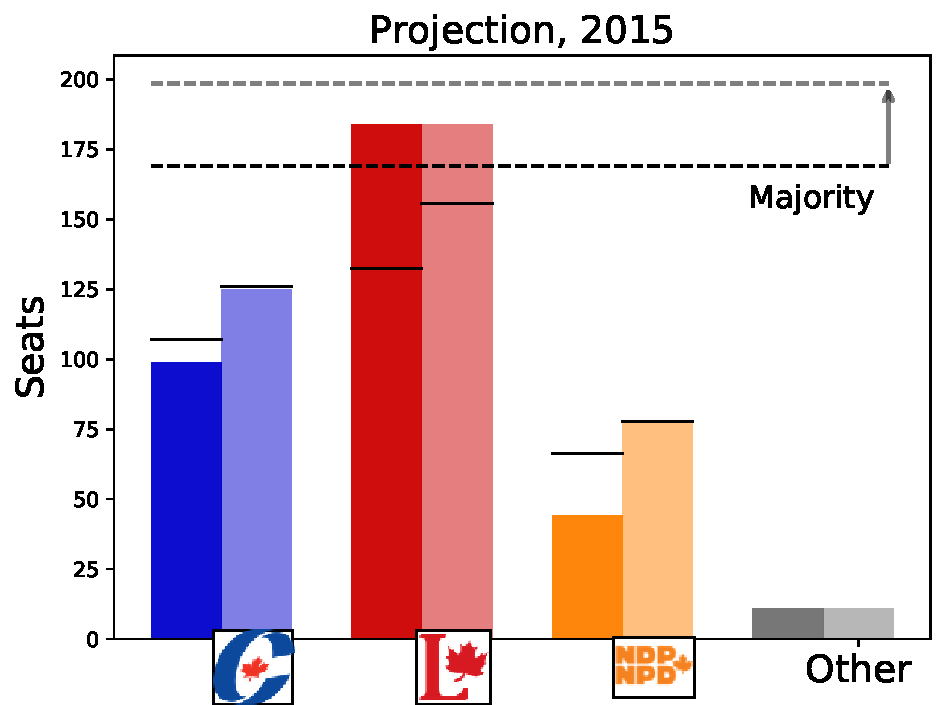
\includegraphics[width=0.50\textwidth,clip]{PR_calcs/data/raw_2015/PMM_out/PMM_projections}
  \caption{ Seat distribution following the 2015 federal election, using the same conventions as in Fig.~\ref{fig:projection_2019}.}
\label{fig:projection_2015}
\end{figure}



%----------------------------------------------------------------------------------------
%	Ceiling Parliament size
%----------------------------------------------------------------------------------------
\section{Extreme Split-Ballot Scenarios}

Data from recent elections indicate that PMM would establish proportional representation with the addition of about 60 supplementary MPs in a typical election, however, we can imagine pathological cases.

Consider the extreme case where an under-represented party, $X$, receives zero \--or few\-- constituency seats, and yet is awarded nearly 100\% of the second-ballot votes.
Of course, this is exceedingly unlikely in practice and would be even more implausible given measures against decoy-lists (see conclusion, main text).
Nevertheless, for this hypothetical scenario a truly proportional legislature would require adding an \emph{infinite} number of supplemental MPs from party \textbf{$X$}.

To avoid this problem, a hard upper limit to supplementary seats must be established \--for example, twice the number of constituencies. In our model, this quantity $\hat N \stackrel{!}{\le} N_{\textrm{max}} = 2 N$ is set as our upper-limit to ensure that constituent MPs are never in the minority, although more conservative constraints (i.e., smaller values of $N_{\textrm{max}}$) are also possible, and have been used in other MM systems.
The general rule remains:

\begin{align}
\label{eq:Nlimits}
N &\le& \hat{N} &\le& N_{\textrm{max}} \\
FPP &\le& PMM &\le& MM
\end{align}

The inequalities above serve to highlight that PMM will entail more seats than FPP, but fewer than traditional MM, as employed in, for example, Germany.
Both the upper and lower limits of this system (i.e., standard FPP and MM models) have been tested and shown practical in a functioning democracy. PMM seeks an optimal combination therein and is constrained to ensure that it can never go beyond the limits of what has been tested and shown to work.

% Finally, the 5\% threshold has been used as a filter of national support to limit supplementary seats to sincere and credible parties.
% The fact that this has the effect of encouraging parties to seek broad-based support throughout the country may be seen as a design feature, promoting national unity, however, it will likely be met with opposition be an established regional party such as the Bloc Quebecois.
% A palatable compromise may be to set the threshold at "5\% support nationally, \emph{or} 10\% support in at least one province...". In practice, the BQ has consistently exceeded this threshold, and the point may be moot.

